\chapter{Características de salida del JFET}
Las características de salida de un JFET describen la relación entre la corriente de drenaje $I_D$ y la tensión
drenaje–fuente $V_{DS}$, para diferentes valores de la tensión puerta–fuente $V_{GS}$. Estas curvas permiten visualizar
el comportamiento del dispositivo en sus distintas regiones de operación: la región óhmica (cuando $V_{DS}$ es bajo y la
corriente aumenta casi linealmente), la región de saturación o activa (cuando $I_D$ se estabiliza para un $V_{DS}$
suficiente), y el corte (cuando $V_{GS}$ es más negativo que $V_{GS(\text{off})}$ y la corriente se anula).

\lipsum[1]

La medición de estas curvas resulta fundamental para caracterizar el transistor, ya que de ellas se puede determinar
experimentalmente parámetros clave como la corriente de saturación $I_{DSS}$, la tensión de estrangulamiento $V_P$ y el
rango de operación útil del dispositivo. En esta sección se presentan los resultados obtenidos en el laboratorio, a
partir de la variación de $V_{DS}$ para distintos valores fijos de $V_{GS}$, construyendo así la familia de curvas
característica del JFET empleado.

  \section{Actividad de Simulación}
    Se propuso implementar el circuito de la figura \ref{crkt:jfet-transf} en el simulador LTSpice, y hacer que la fuente
    $V1$ varíe desde $0V$ a $8V$ en pasos de $0.1V$, y por cada variación de la fuente $V1$, que la fuente $V2$ varíe de
    $0V$ a $15V$ en pasos de $0.1V$ para poder recrear una familia de curvas que expongan el comportamiento de la
    corriente $I_D$ en función del voltaje drain-source $V_{DS}$ por cada $V_{GS}$.
    \begin{figure}[!ht]
      \centering
      \begin{minipage}{0.45\textwidth}
        \begin{tikzpicture}
          % Paths, nodes and wires:
          \node[njfet](N1) at (2.25, 2.73){} node[anchor=west] at (N1.text){$2N5457$};
          \draw (4.75, 3.48) to[battery, l={$V2$}] (4.75, 1.98);
          \draw (4.75, 3.46) -- (4.75, 5.21) |- (2.25, 5.21) -| (2.25, 3.48);
          \draw (2.25, 1.96) -- (2.25, 0.73);
          \draw (4.75, 1.98) -- (4.75, 0.73);
          \node[ground] at (0.25, 0.73){};
          \node[ground] at (2.25, 0.73){};
          \node[ground] at (4.75, 0.73){};
          \draw (0.25, 1.25) to[battery, l={$V1$}] (0.25, 2);
          \draw (1.27, 2.46) -| (0.25, 2);
          \draw (0.25, 0.73) -| (0.25, 1.25);
        \end{tikzpicture}
        \caption{circuito de prueba para características de transferencia.}
        \label{crkt:jfet-sal}
      \end{minipage}
      \hfill
      \begin{minipage}{0.45\textwidth}
        \begin{lstlisting}[style=ltspice, caption={Parámetros de simulación LTspice}, label=list:jfet-transf]
.MODEL 2N5457 NJF IS=1N VT0=-1.5 BETA=1.125M LAMBDA=2.3M CGD=4PF CGS=5PF
.dc V2 0 15 .1 V1 0 8 .1
        \end{lstlisting}
      \end{minipage}
    \end{figure}

    \begin{figure}[!ht]
      \centering
      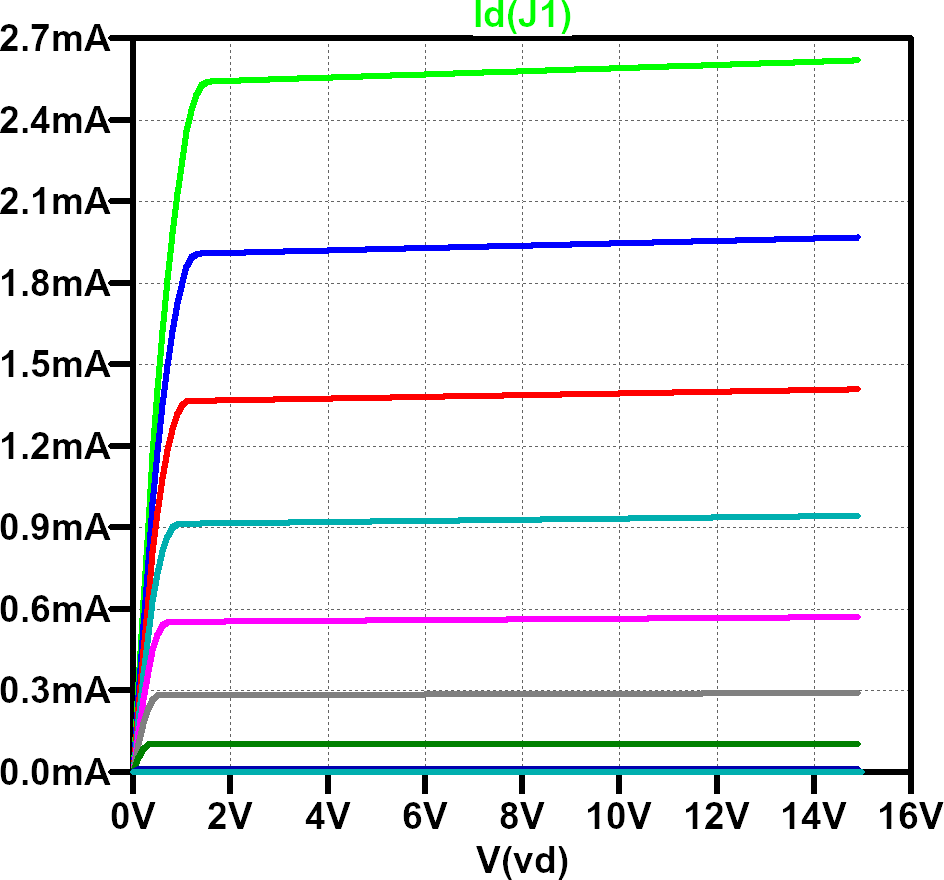
\includegraphics[width=0.65\textwidth]{images/salida-id_vds-vgs.png}
      \caption{resultados de simulación para características de salida del JFET.}
      \label{fig:sim.sal}
    \end{figure}

    Para poder apreciar mejor los resultados de la figura \ref{fig:sim.sal}, se redujo el barrido de la fuente $V1$
    hasta $3V$ en pasos de $0.2V$. Como se puede ver, el modelo describe perfectamente la familia de curvas de
    $I_{D_{(V_{DS}, \, V_{GS}})}$. La única diferencia observable comparada con la gráfica presentada por el fabricante es el
    valor de $I_{DSS}$.

\section{Actividad de Laboratorio}

    En esta actividad se implementó el circuito que se nos planteo con el objetivo de obtener las curvas características
    $I_{DS} = f(V_{DS})$ para distintos valores de $V_{GS}$.  El procedimiento consistió en fijar un valor de $V_{GS}$,
    variar la tensión $V_{DS}$ y medir los correspondientes valores de $I_{DS}$. Posteriormente, se cambió el valor de
    $V_{GS}$ y se repitió la medición, obteniendo así diferentes curvas que permiten observar el efecto del voltaje de
    compuerta en la corriente de drenaje.  
    
    \begin{figure}[H]
    \centering
    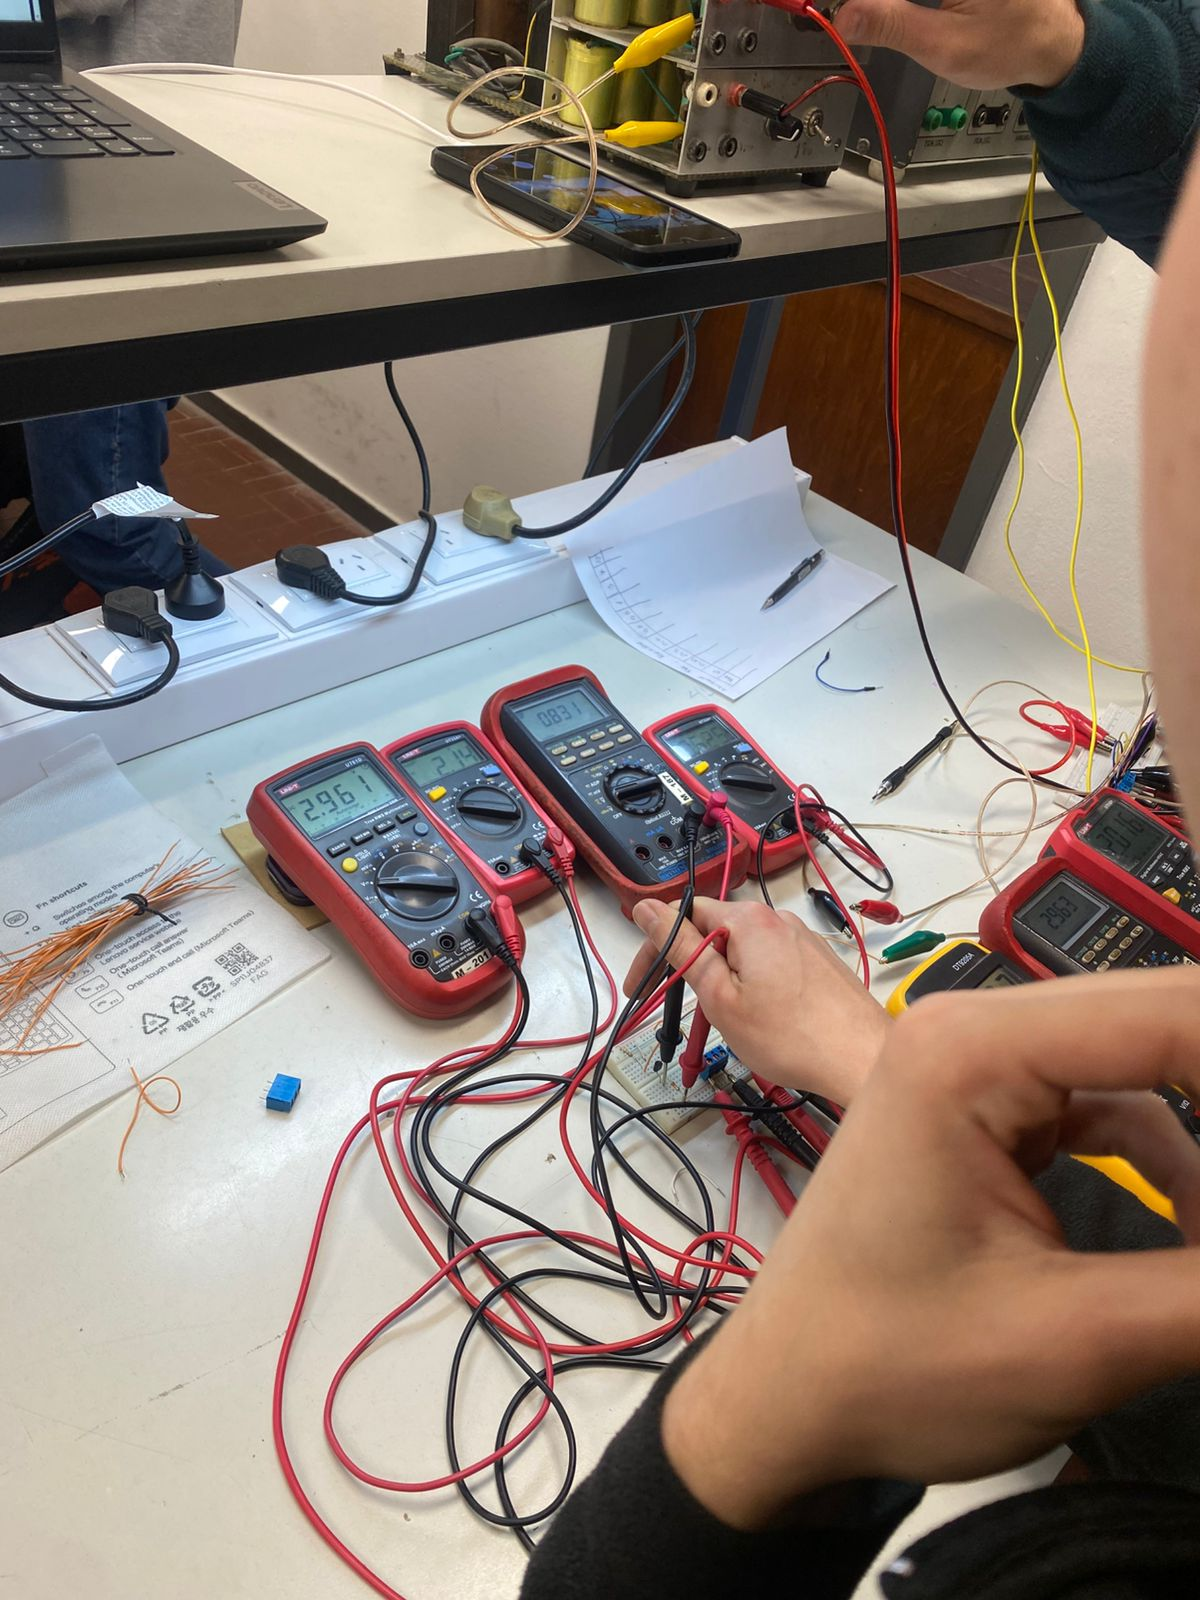
\includegraphics[width=0.5\textwidth]{pictures/robada-tp3.jpeg}
    \caption{Circuito utilizado para la medición de $I_{DS} = f(V_{DS})$ para distintos $V_{GS}$.}
    \label{fig:jfet-carac}
    \end{figure}
    
    Los valores experimentales obtenidos se resumen en la siguiente tabla:
    
    \begin{table}[H]
    \centering
    \resizebox{\textwidth}{!}{%
    \begin{tabular}{|c|c|c|c|c|}
    \hline
        \textbf{$V_{DS}$ [V]} & \textbf{$I_D$ [mA] ($V_{GS}=0$ V)} & \textbf{$I_D$ [mA] ($V_{GS}=-0.1$ V)} & \textbf{$I_D$ [mA] ($V_{GS}=-0.2$ V)} & \textbf{$I_D$ [mA] ($V_{GS}=-0.3$ V)}\\ \hline
    0  & 0    & 0    & 0    & 0    \\ \hline
    1  & 0.84    & 0.32    & 0.05    & 2.6    \\ \hline
    2  & 0.98 & 0.39 & 0.07  & 4.3 \\ \hline
    3  & 1.1    & 0.46    & 0.09    & 6.1    \\ \hline
    4  & 1.14 & 0.52  & 0.12 & 8.5  \\ \hline
    5  & 1.31    & 0.57    & 0.137    & 10.1    \\ \hline
    6  & 1.39 & 0.62 & 0.155 & 12.3 \\ \hline
    7  & 1.47    & 0.67    & 0.172    & 15.5    \\ \hline
    8  & 1.59 & 0.73  & 0.146  & 18.3 \\ \hline
    9  & 1.64    & 0.77    & 0.211    & 21.5    \\ \hline
    10 & 1.72 & 0.83 & 0.212  & 25.5 \\ \hline
    \end{tabular}}
    \caption{Valores de $I_{DS}$ en función de $V_{DS}$ para distintos valores de $V_{GS}$.}
    \label{tab:ids-vds-vgs}
    \end{table}
    
    A partir de estos resultados es posible traficar el conjunto de curvas características del transistor y compararlas
    con las simulaciones y los valores obtenidos de la hoja de datos del fabricante.
    
